
%% bare_jrnl.tex
%% V1.3
%% 2007/01/11
%% by Michael Shell
%% see http://www.michaelshell.org/
%% for current contact information.
%%
%% This is a skeleton file demonstrating the use of IEEEtran.cls
%% (requires IEEEtran.cls version 1.7 or later) with an IEEE journal paper.
%%
%% Support sites:
%% http://www.michaelshell.org/tex/ieeetran/
%% http://www.ctan.org/tex-archive/macros/latex/contrib/IEEEtran/
%% and
%% http://www.ieee.org/



% *** Authors should verify (and, if needed, correct) their LaTeX system  ***
% *** with the testflow diagnostic prior to trusting their LaTeX platform ***
% *** with production work. IEEE's font choices can trigger bugs that do  ***
% *** not appear when using other class files.                            ***
% The testflow support page is at:
% http://www.michaelshell.org/tex/testflow/


%%*************************************************************************
%% Legal Notice:
%% This code is offered as-is without any warranty either expressed or
%% implied; without even the implied warranty of MERCHANTABILITY or
%% FITNESS FOR A PARTICULAR PURPOSE! 
%% User assumes all risk.
%% In no event shall IEEE or any contributor to this code be liable for
%% any damages or losses, including, but not limited to, incidental,
%% consequential, or any other damages, resulting from the use or misuse
%% of any information contained here.
%%
%% All comments are the opinions of their respective authors and are not
%% necessarily endorsed by the IEEE.
%%
%% This work is distributed under the LaTeX Project Public License (LPPL)
%% ( http://www.latex-project.org/ ) version 1.3, and may be freely used,
%% distributed and modified. A copy of the LPPL, version 1.3, is included
%% in the base LaTeX documentation of all distributions of LaTeX released
%% 2003/12/01 or later.
%% Retain all contribution notices and credits.
%% ** Modified files should be clearly indicated as such, including  **
%% ** renaming them and changing author support contact information. **
%%
%% File list of work: IEEEtran.cls, IEEEtran_HOWTO.pdf, bare_adv.tex,
%%                    bare_conf.tex, bare_jrnl.tex, bare_jrnl_compsoc.tex
%%*************************************************************************

% Note that the a4paper option is mainly intended so that authors in
% countries using A4 can easily print to A4 and see how their papers will
% look in print - the typesetting of the document will not typically be
% affected with changes in paper size (but the bottom and side margins will).
% Use the testflow package mentioned above to verify correct handling of
% both paper sizes by the user's LaTeX system.
%
% Also note that the "draftcls" or "draftclsnofoot", not "draft", option
% should be used if it is desired that the figures are to be displayed in
% draft mode.
%
\documentclass[journal]{IEEEtran}

\usepackage{graphicx}
\usepackage{balance}


% *** CITATION PACKAGES ***
%
%\usepackage{cite}
% cite.sty was written by Donald Arseneau
% V1.6 and later of IEEEtran pre-defines the format of the cite.sty package
% \cite{} output to follow that of IEEE. Loading the cite package will
% result in citation numbers being automatically sorted and properly
% "compressed/ranged". e.g., [1], [9], [2], [7], [5], [6] without using
% cite.sty will become [1], [2], [5]--[7], [9] using cite.sty. cite.sty's
% \cite will automatically add leading space, if needed. Use cite.sty's
% noadjust option (cite.sty V3.8 and later) if you want to turn this off.
% cite.sty is already installed on most LaTeX systems. Be sure and use
% version 4.0 (2003-05-27) and later if using hyperref.sty. cite.sty does
% not currently provide for hyperlinked citations.
% The latest version can be obtained at:
% http://www.ctan.org/tex-archive/macros/latex/contrib/cite/
% The documentation is contained in the cite.sty file itself.


\begin{document}


\title{A Proof of Concept Parser for the Montery-Phoenix Modeling Language}


\author{Steve Mazza% <-this % stops a space
\thanks{S. Mazza is a student in the Department of Systems Engineering at the 
Naval Postgraduate School, Monterey, CA, 93943-5100 USA 
e-mail: spmazza@nps.edu.}% <-this % stops a space
}


\maketitle


\begin{abstract}
Encouraging the use of and enhancing accessibility to the 
Monterey-Phoenix (MP) systems engineering modeling language requires the
development of tools to streamline work-flow and facilitate visualization.
Here we lay the foundation for the development of a parser for the
MP language which will allow us to verify the syntax of a given MP source file. 
This is the first step in preparation of a semantically equivalent graphical
representation of the model.
\end{abstract}


\begin{IEEEkeywords}
    Monterey-Phoenix, systems engineering, language, parser, compiler.
\end{IEEEkeywords}


\IEEEpeerreviewmaketitle


\section{Introduction}

\IEEEPARstart{E}{ncouraging} the use of and enhancing accessibility to the 
Monterey-Phoenix (MP) systems engineering modeling language requires the
development of tools to streamline work-flow and facilitate visualization. 
Ideally, constructs written in an editor with proper syntax would be 
represented as a graph showing structure, dependencies, and state transitions.
This aids the programmer both in the verification of correctness of the 
semantics and in the communication of ideas to the non-programmer.

The real power, however, occurs in the generation of semantically and syntactically
correct grammar from a manual alteration, enhancement, or arrangement of 
the graphical representation of the model, thereby empowering the non-programmer
to unlock the full potential of the powerful systems engineering modeling
language.  Providing an automated textual representation of the model also
ensures that work products can be managed in a complex and integrated team
setting with mature version control systems such as Git and Subversion.

Here we lay the foundation for the development of a parser for the
MP language which will allow us to verify the syntax of a given MP source file. 
This is the first step in preparation of a semantically equivalent graphical
representation of the model.  We will not be creating the graphical model, nor will we
be addressing a means to update source code based on manual alterations to the
graphical model.  These are opportunities for future work.

\hfill spm
 
\hfill March 05, 2014

\section{Process}
The first step to parsing the file is to take the contents (text) of the 
MP source code file and perform a lexical analysis
to break the input into tokens.  These tokens are sub-strings in the file that 
represent the keywords, operators, variables, constants, and other valid syntax 
items of the language.  Comments are normally ignored.

The tokens are then fed to the parser which produces either a parse tree or an error.
A parse tree is a semantic-preserving graphical representation of the syntax contained
in the source file and represented by the tokens coming from the lexical analyzer.  You 
might notice that this parse tree, while only an abstract data structure, will likely provide an
easy way to produce a visually appealing graph of the MP model at some future point.


\subsection{Lex and Yacc}
Lex and yacc (or flex and bison\footnote{\emph{Flex} and \emph{bison}
are common modern implementations of lex and yacc.}) 
are standard POSIX tools for performing lexical analysis (parsing) and compilation.
They are very handy, well documented, and are part of most standard 
Unix-like distributions (e.g., Linux, FreeBSD) and are 
also included in OS X.  There are also many publicly available examples of how to use these
tools which provide good starting points for new work.  We rely on these along with the
configuration file to generate our parse tree.


\subsection{Overview of Operation}


\subsubsection{Lex (the Lexical Analyzer)}
The first step in using lex and yacc together is to create a patterns file that helps lex
correctly identify tokens within source code.  The easiest way to do this is to write 
regular expressions that catch the language tokens and filter out comments.  These
regular expression are the main part of the lex input file and specify patterns
and their corresponding actions.  The patterns are written using an extended set 
of regular expression syntax.  The regular expressions are implemented using a 
greedy match approach, attempting to match as much text as possible.  

The file containing the regular expressions is fed to lex which produces a C-code source
file that can either be compiled into a stand-alone parser or used (as we will see shortly)
along with a similar file generated by yacc to create an end-to-end parser-compiler.  
Whenever patterns are updated, lex needs to be called in order to re-process the file.

Either way, once the parser is created we are done with lex.  The parser takes an input
stream consisting of the target language source code.  It identifies language tokens within
the stream and by default returns  the token type for everything it finds.  This is interesting
by itself but when coupled with yacc becomes very powerful.

\begin{center}
\begin{figure}[htb]
	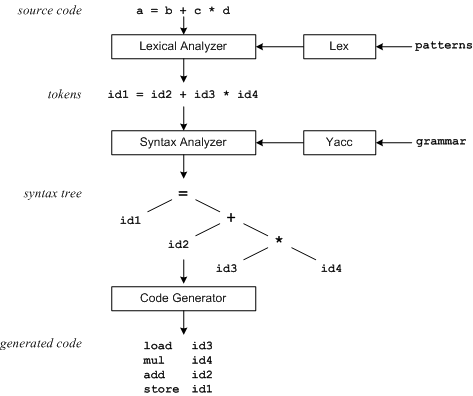
\includegraphics[width=\columnwidth]{fig11.png}
	\caption{\label{fig:lex-yacc}Lex-yacc interaction.}
\end{figure}
\end{center}


\subsubsection{Yacc (Yet Another Compiler Compiler)}
In a similar manner, yacc takes a configuration file and generates C-code source which
is usually compiled along with the lex C-code into a complete parser-compiler.  The yacc 
configuration file is a context free grammar describing the language.  Yacc does not 
understand the source code file stream and needs lex to parse the stream into tokens that
it can look up within the supplied grammar.  Conversely, lex can recognize tokens within a file
stream but does not know what to do with them apart from passing them on to yacc.

While yacc has traditionally been used to create compilers, it can be made to return anything
at all.  The tokens received from lex are stored in a parse tree which can be traversed and
used to syntactically check for errors, generate source code in another language, 
generate a graphical representation of the parse tree, or anything else of utility.  All
that is required is to write the correct C-code in the configuration file to affect the 
desired output.

Figure \ref{fig:lex-yacc} shows the classical example of the interaction of lex, yacc, and
their respective configuration files, the source code input, and a typical resulting output.

\balance
\section{Conclusion}
I believe that lex and yacc represent a proven and well documented approach to creating
a parser-compiler for the Monterey-Phoenix language.  They are available on most 
modern operating systems and require only a working knowledge of regular expression,
C, and a description of the grammar in which you want to work.

Using a coordinated approach with these two tools yields a far greater return on effort than
designing a solution from scratch.  Furthermore, the flexibility in tailoring your output
by writing handlers in C means that the source file can be transformed in almost any 
way imaginable.  While these tools are not as commonly used as they once were, they remain
readily accessible and can be easily installed on almost any operating system.

All of these factors combine to make a powerful approach to providing increased utility and
accessibility to the Monterey-Phoenix language.  I would like to encourage the pursuit of 
an implementation of the full grammar which would not only provide a native MP compiler
on every operating system but would also provide the basis for building an interactive
graphical editor.


\appendix[Acknowledgment]
The author would like to thank Dr. Giammarco and Dr. Auguston 
for their direction and support.


% references section
%


% biography section
% 

\begin{IEEEbiographynophoto}{Steve Mazza}
is a graduate student at the Naval Postgraduate School in Monterey, CA, and
is employed by the US Army where he leads the systems engineering effort for the 
development of a prototype Mission Command variant of a Ground Combat System.
\end{IEEEbiographynophoto}


\end{document}


